\documentclass{article}
\usepackage{parskip}
\usepackage[margin=1.5cm]{geometry}
\usepackage{graphicx}
\usepackage{framed}
\usepackage{float}
\usepackage{listings}

\graphicspath{{.}}

% Thanks to Angus Pearson for nagging me to fuck about with fonts in
% XeLaTeX

\usepackage{fontspec} \usepackage{xltxtra}

% PT Serif
\setromanfont[ BoldFont=PTF75F.ttf, ItalicFont=PTZ56F.ttf,
BoldItalicFont=PTF76F.ttf, ]{PTF55F.ttf}

% Noto Sans
\setsansfont[ BoldFont=NotoSans-Bold.ttf,
ItalicFont=NotoSans-Italic.ttf, BoldItalicFont=NotoSans-BoldItalic.ttf
]{NotoSans-Regular.ttf}

\begin{document}

\textbf{\Huge Operating Systems Notes}

\section{OSs and Architectures}

Different architectures dictates the way that an operating system must conduct its business.

As different architecture platforms have different instruction sets, it determines what are viable methods for accomplishing tasks such as \textit{memory protection} and \textit{control interrupts}.

The OS acts as an intermediary between software and hardware. It allows to mediate access and gives developers a nicer way of completing lower-level actions. This abstraction is achieved via \textit{traps} and \textit{exceptions}. Similarly, devices can gain attention via the use of \textit{interrupts}.

An OS is intended to be a good balance between \textit{user needs} and \textit{system needs}.

A user wants an OS to be \textit{fast, reliable and safe}; an OS developer wants it to be \textit{efficient, error-free, and easy to maintain and implement}.

The design of an operating systems makes a distinction between two underlying principles:

\textbf{Policy}, which is \textit{what} will be done; \textbf{Mechanism}, which his \textit{how} to do it.

\subsection{Structure of an OS}

A capable operating system is home to a multitude of components: memory management, I/O, file systems, command interpreters and so on. There are multiple ways to link to structure how all these components are connected to each other.

\subsubsection{Monolithic}

An early type of design for an OS, where the \textit{entire} operating system would function in \textit{kernel mode} (see the \textit{Privileged Instructions} section). However, this design carried many issues with maintainability and reliability, and was hard to make sense of.

\subsubsection{Layering}

As opposed to monolithic, this method implemented the OS as a \textit{set of layers} instead, where a layer could present itself to the corresponding layer above.

\begin{figure}[H]
  \centering
  \begin{center}
  \begin{tabular}{|c|c|l|}
    \hline
    5 & \textbf{Job Managers} & Execute a user's programs\\
    \hline
    4 & \textbf{Device Managers} & Handle devices, provide buffering\\
    \hline
    3 & \textbf{Console Manager} & Provide virtual consoles\\
    \hline
    2 & \textbf{Page Manager} & Implement virtual memories for each process\\
    \hline
    1 & \textbf{Kernel} & Implement a virtual processor for each process\\
    \hline
    0 & \textbf{Hardware} & \\
    \hline
  \end{tabular}
\end{center}
\caption{Dijkstra's THE System}
\end{figure}

\filbreak
\subsection{Privileged Instructions}

These instructions are restricted to use by the OS \textit{only}, and includes direct access to \textit{I/O devices} and \textit{memory state management}.

This is achieved by the implementation of two \textit{modes of operation}; \textit{user} and \textit{kernel} modes.

Privileged instructions can only be executed in kernel mode.

\begin{figure}[h!]
  \centering
  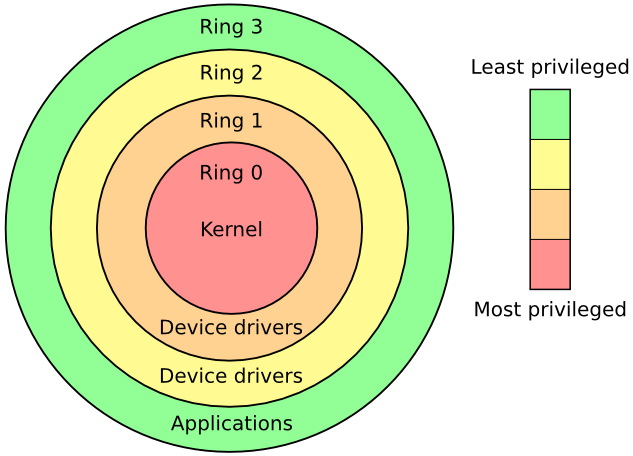
\includegraphics[scale=0.35]{privilegeGraphX86}
  \caption{x86 Architecture Levels of Privilege}
  \textit{\footnotesize Courtesy of Hertzsprung of English Wikipedia}
\end{figure}

\subsubsection{System Calls}

If code running from within user mode tries to execute a privileged instruction, it will trigger the \textit{illegal execution trap}, which allows for such code to gain access to privileged instructions and resources. These are called \textit{system calls}.

An OS will define a set of system calls that makes it possible for such an interaction to take place.

\begin{figure}[H]
  \begin{framed}
    \textit{Caller}: The user mode process invoking the system call\\
    \textit{Callee}: The OS handling the system code\\
    \begin{itemize}
    \item The caller places arguments, especially the \textit{type} of system call, in a specified location
    \item The callee saves the caller's state
    \item The callee verifies the arguments
    \item If valid, the code is run
    \item When the system call has been satisfied, the program counter is set to the return address
    \item Execution is returned to user mode
    \end{itemize}
  \end{framed}
  \caption{A rough breakdown of a system call}
\end{figure}

\subsection{Exception Handling}

A \textit{trap} is a synchronised, intended transition that is initiated by the OS.

An \textit{exception} is also synchronised, however it is an \textit{unexpected} problem with some instruction.

An \textit{interrupt} is \textit{a}synchronous on the other hand, and is caused by some external device.




\filbreak
\section{Memory Management}
Programs must be brought from disk into mmemory and then placed into a process.

The CPU can only access data from memory, not disk.

Register access takes at most 1 CPU clock, but Main Memory can take mayn cycles, causing a \emph{Stall}.

\subsection{Base and Limit Registers}
A set of \emph{base} and \emph{limit registers} define the logical adress space. the CPU must chech every
memory access is valid between the base and the limit for that user. Failure causes a trap to the OS monitor

\subsection{Virtual Address Space}
Logical/Virtual addresses are independent of physical memory.

Hardware translates virtual addresses into physical ones.

Logical/Virtual addresses a process can reference is called the address space.

\subsection{Memory Managment Unit (MMU)}
Effectively is a hash function from logical address to physical address.

a MMU prevents the need for swapped out process to be swapped back into the same physical addresses.

Swapping is not typically supported on mobile devices, more likely to to overwite least used data.


\subsection{Partitioning}
Main memory is usually broken up into two partitions; The OS and user process.

Each process is contained within a single contiguous section on memory.

Realocation registers are used to protect users processes from one another and from canging the OS code.

Some old techniques include:
\begin{itemize}
    \item Fixed Partitions - simple but causes fragmentation often
    \item Variable Partitions - no internal fragmentation, but can leave holes in the physical memory
\end{itemize}

Dynamic Storage-Allocation is possible using First-fit, Best-fir and Worst-fit in terms of hole filling.




\filbreak
\section{MutEx}\label{mutex}

A \emph{critical section} is a sequence of code that may result in
incorrect or undefined behaviour if executed simultaneously or
preempted. Similarly, race conditions occur when the order of execution
is unknown and behaviour can be unpredictable.

Mutual Exclusion (MutEx) and locking prevent these problems.

To be safe and operate correctly, a critical section must satisfy the
following requirements:

\begin{description}
\item[Mutual Exlusion]
At most one thread is in the critical section
\item[Progress]
If a thread is outside the critical section, it cannot prevent another
from entering
\item[Bounded Waiting \& No Starvation]
If a thread is waiting to enter the critical section, it is guaranteed
to eventually do so
\item[Performance]
The overhead of entering and exiting the critical section is small
relative to the runtime of the section.
\end{description}

\begin{figure}[h!]
  \centering
  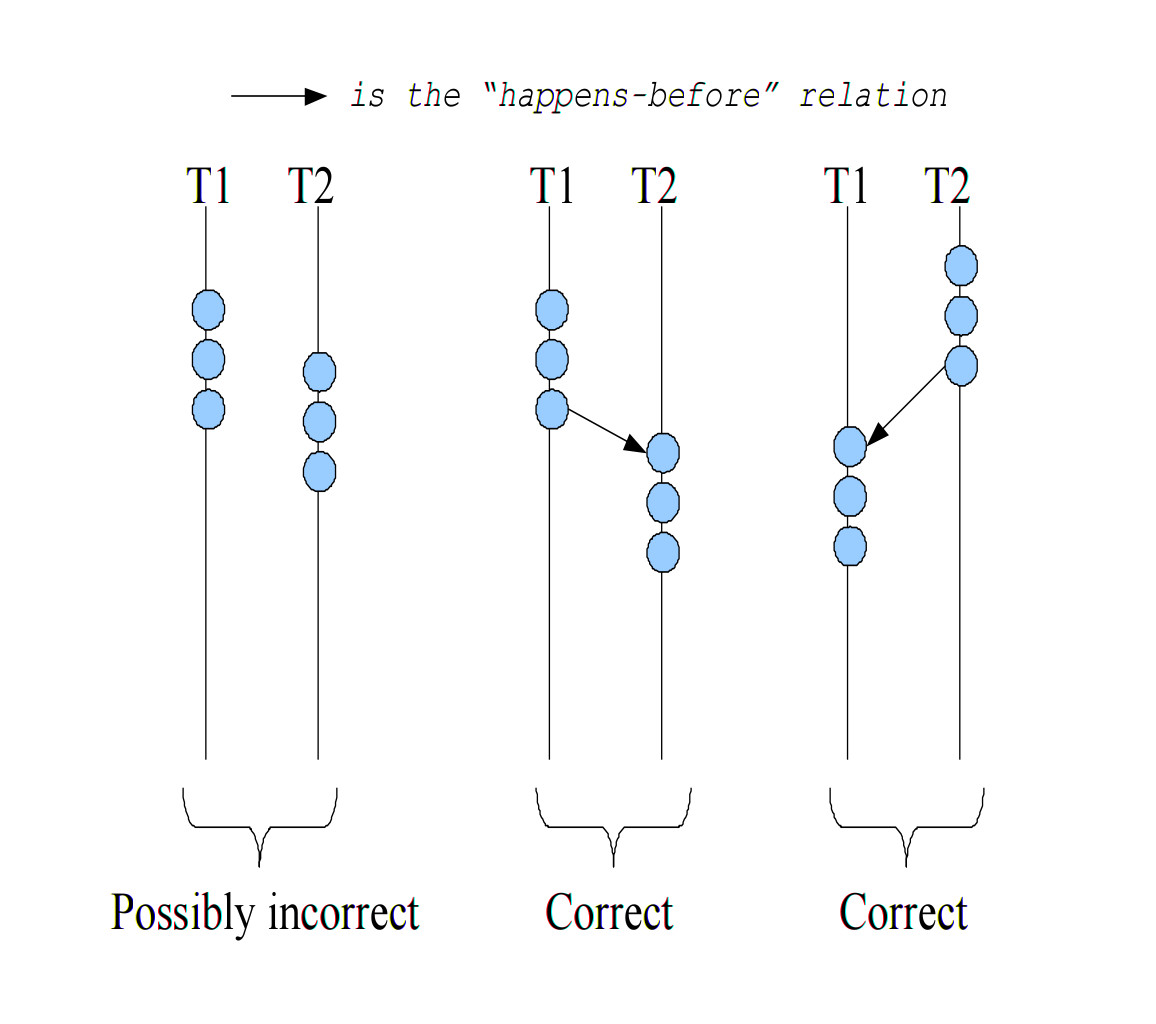
\includegraphics[width=0.5\textwidth]{correctConcurrency}
  \caption{Concurrency Dependencies}
\end{figure}


\subsection{Peterson's Algorithm}\label{petersons-algorithm}

\begin{verbatim}
flag[i] = True;
turn = 1-i;

while (flag[1-i] && turn == 1-i); // spin

/* critical section code */

flag[i] = False;
\end{verbatim}

Avoids both \emph{deadlock} and \emph{livelock} for two threads, using
\texttt{i} and \texttt{i-1} as signals. It works but can be tricky to
implement.

\subsection{Spinlocks}\label{spinlocks}

A \textbf{spinlock} is a locking primative, used to build more complex
locking mechanisms. The name comes from the behaviour; It `spins' on a
condition until it is satisfied, so will acquire the lock as soon as it
is available.

\begin{verbatim}
// do not have lock
while(some_condition);
// have lock
\end{verbatim}

Acquiring and releasing locks \emph{must} be an atomic operation, so no
contect switching occurs during acquisition which could lead to a crash
or undefined state. \textbf{Test and Set} is an atomic instruction we
can use to acheive this.

\begin{verbatim}
struct spinlock{
    int held;
};

struct spinlock lock;
lock.held = 0;

int test_and_set(int* flag){
    int old = *flag;
    flag = 1;
    return old;
}

void acquire(struct lock* lock)
{
    /* This is the `spinning' */
    while(test_and_set(&lock->held));
}

void release(struct lock* lock)
{
    lock->held = 0;
}
\end{verbatim}

Spinlocks are simple to implement, but can be slow and \emph{block}
whilst waiting for the lock, wasting CPU time.

\subsection{Semaphores}\label{semaphores}

Similar to a spinlock, having the two operations
\texttt{wait(semaphore)} and \texttt{signal(semaphore)}, sometimes given
as \texttt{P(semaphore)} and \texttt{V(semaphore)}. Semaphores can use
integer signals, or a boolean - the boolean semaphore has the same
behaviour as a lock.

\begin{verbatim}
void wait(semaphore s)
{
    while(s <= 0); // Busy wait
    s--;
}

void signal(semaphore s)
{
    s++;
}
\end{verbatim}

This simple implementation uses \emph{busy waiting}. We can use a wait
queue instead, placing ourselves onto the queue and yielding until the
semaphore is available.

\begin{verbatim}
void wait(semaphore* s)
{
    s->value--;
    if(s->value < 0){
        enqueue_process();
        /* Add self to the wait queue and block/sleep */
    }
}

void signal(semaphore* s)
{
    s->value++;
    if(s->value <= 0){
        dequeue_process();
        /* Remove a process from the wait queue and wake it */
    }
}
\end{verbatim}

\subsubsection{Bounded Buffer Problem}\label{bounded-buffer-problem}

In a \textbf{producer and consumer} model, we can have many threads
wishing to consume some data, and many that produce it. The handover of
data can be done with a \emph{bounded buffer}

\begin{figure}[h!]
  \centering
  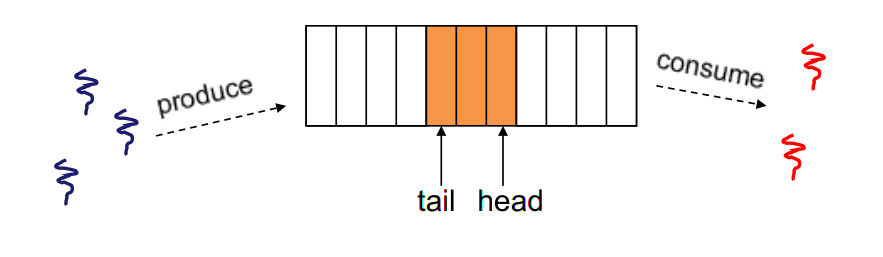
\includegraphics[width=0.8\textwidth]{produceConsume}
  \caption{Producer-Consumer model}
\end{figure}


We can use three semaphores to ensure safety around this bounded buffer:

\begin{tabular}{l | c | l }
mutex & 1 & Mutual exlusion on shared data (head \& tail\ldots{})\\
empty & n & Number of empty / available slots in the buffer. Initially all available.\\
full  & 0 & Number of taken slots in the buffer. Initially none are taken.
\end{tabular}

\begin{verbatim}
producer:
    wait(empty)
    wait(mutex)
        add item to buffer
    signal(mutex)
    signal(full)

consumer:
    wait(full)
    wait(mutex)
        remove item from buffer
    signal(mutex)
    signal(empty)
\end{verbatim}

\subsubsection{Pub Sub}\label{pub-sub}

The constraints on \textbf{publishers} (aka writers) and
\textbf{subscribers} (aka readers) are different:

\begin{enumerate}
\item
  We \emph{can} allow multiple subscribers to concurrently access
\item
  We \emph{cannot} allow publishers and subscribers to concurrently
  access
\item
  We \emph{cannot} have more than one publisher concurrently writing
\end{enumerate}

This is because subscribers make the promise to not mutate the data,
while publishers do not.

\begin{tabular}{l | c | l }
semaphore: mutex     & 1 & Mutual exlusion on shared data\\
semaphore: writing   & 1 & Lock on mutation/writing to the data\\
integer: read\_count & 0 & The number of subscribers currently reading
\end{tabular}

\begin{verbatim}
writer:
    wait(writing)
        perform writes // Satisfies requirement 3
    signal(writing)
    
reader:
    wait(mutex)
        reader_count++;
        if (reader_count == 1) wait(writing); // Satisfy requirement 2
    signal(mutex)
    
    do reading
    
    wait(mutex)
        reader_count--;
        if (reader_count == 0) signal(writing); // Release lock on writers if no further readers
    signal(mutex)
\end{verbatim}


\subsection{Condition Variables}

Has similar operations to Semaphores: \texttt{wait()} and \texttt{signal()}.

\begin{description}
  \item[Wait] Wait until another thread has signaled and released the lock
  \item[Signal] Wake a thread from the wait queue
\end{description}

Signals aren't remembered if there are no threads in the wait queue like they are with semaphores.

\subsubsection{Bounded Buffer}


\begin{tabular}{l | c | l }
lock:      mutex    & 1 & Mutual exlusion on shared data (head \& tail\ldots{})\\
condition: freeslot & n & There is at least one slot free\\
condition: fullslot & 0 & There is at least one slot taken
\end{tabular}

\begin{verbatim}
producer:
    lock(mutex)
    if [no slots available] wait(freeslot);
        Add item...
    signal(fullslot)
    unlock(mutex)

consumer:
    lock(mutex)
    if [no slots have data] wait(fullslot);
        Pop item from shared buffer
    signal(freeslot)
    unlock(mutex)
    Use item...
\end{verbatim}

\subsection{Possible Bugs}

Most locking mechanisms are prone to bugs; They're shared data structures, and there's never a
guarantee a logck will ever be released or acquired when it should be.

The lock is also not strictly associated with the data it protects; Have we got the right lock? 
Should we have more than one lock? Programming language structures
such as classes with built in locking mechanisms go some way to protect against these errors.


\subsection{Monitors}

A higher level programming language structure, requires some notion of objects (so would be tricky 
in C, much easier in C++). Each method in the class automatically acquires a lock on entry, 
releasing it on exit. This is transparent to the implementer of the API exposed by the class. 
Safeties that come from using classes, such as protected/private methods and structures help protect data.

Implementation of a monitor class in C++. \verb|invariant| is asserted over the life of a class, throwing an
error if the condition is broken. Similarly \verb|precondition| asserts a condition before method
execution is allowed. 

\begin{verbatim}
class Account {
  private lock myLock;

  private int balance := 0
  invariant balance >= 0

  public method boolean withdraw(int amount)
     precondition amount >= 0
  {
    myLock.acquire();
    try:
      if balance < amount then return false
      else { balance := balance - amount ; return true }
    finally:
      myLock.release();
  }

  public method deposit(int amount)
     precondition amount >= 0
  {
    myLock.acquire();
    try:
      balance := balance + amount
    finally:
      myLock.release();
  }
}
\end{verbatim}
\emph{Hoiked from wikipedia, https://en.m.wikipedia.org/wiki/Monitor\_(synchronization)}



\end{document}
